
\subsubsection{ Nguyên lý hoạt động}
Tác vụ "Humidity and Network-Driven NeoPixel Control" chịu trách nhiệm điều khiển đèn LED RGB (NeoPixel) để phản ánh trực quan tình trạng độ ẩm không khí và trạng thái kết nối mạng của hệ thống. Tương tự như LED1, dải NeoPixel cũng hỗ trợ hai chế độ hoạt động: \textit{Auto Mode} và \textit{Manual Mode}.

\begin{itemize}
    \item \textbf{Manual Mode (Chế độ thủ công):} Khi \texttt{led\_auto\_mode} bị tắt, màu sắc của NeoPixel được xác định bởi các giá trị \texttt{led\_manual\_r}, \texttt{led\_manual\_g}, \texttt{led\_manual\_b} và được tinh chỉnh độ sáng thông qua biến \texttt{led\_brightness} (tính theo phần trăm). Sau khi cập nhật màu sắc, vòng lặp sẽ tạm nghỉ 150ms.
    \item \textbf{Auto Mode (Chế độ tự động):} Ở chế độ này, hệ thống sẽ ưu tiên kiểm tra trạng thái kết nối mạng, sau đó mới đánh giá dữ liệu độ ẩm ($H$) từ cảm biến. Các mức hiển thị màu sắc được quy định cụ thể như sau:
    \begin{itemize}
        \item \textbf{Mất kết nối Wi-Fi} (\texttt{!isWifiConnected}): Đèn hiển thị màu Tím (Purple) cảnh báo mất mạng độc lập với dữ liệu cảm biến.
        \item $H \le 60\%$: Độ ẩm lý tưởng, đèn hiển thị màu Xanh lá (Green).
        \item $60\% < H \le 80\%$: Độ ẩm hơi cao, đèn hiển thị màu Đỏ (Red).
        \item $H > 80\%$: Độ ẩm bão hòa, đèn hiển thị màu Xanh dương (Blue).
    \end{itemize}
    Tác vụ chạy với chu kỳ delay là 300ms để đảm bảo cập nhật trạng thái liên tục mà không tiêu tốn tài nguyên hệ thống.
\end{itemize}

\subsubsection{Cơ chế đồng bộ bằng FreeRTOS Semaphore}
Tác vụ \texttt{neo\_blinky} sử dụng hàm \texttt{xSemaphoreTake} để kiểm tra việc có hay không dữ liệu mới từ cảm biến. Khi nhận được Semaphore từ Task đọc cảm biến, biến cục bộ \texttt{local\_hum} sẽ được cập nhật bằng giá trị mới nhất từ biến toàn cục \texttt{glob\_humidity}. Điều này giúp vòng lặp của NeoPixel không bị chặn lại nếu cảm biến chưa đọc xong, duy trì khả năng cảnh báo mất Wi-Fi tức thời. Hệ thống cũng áp dụng kỹ thuật so sánh cờ \texttt{currentColor} và \texttt{newColor} để chỉ gọi hàm \texttt{strip.show()} khi thực sự có sự thay đổi màu sắc,

\subsubsection{Sơ đồ máy trạng thái (FSM)}

\begin{figure}[H]
\centering
    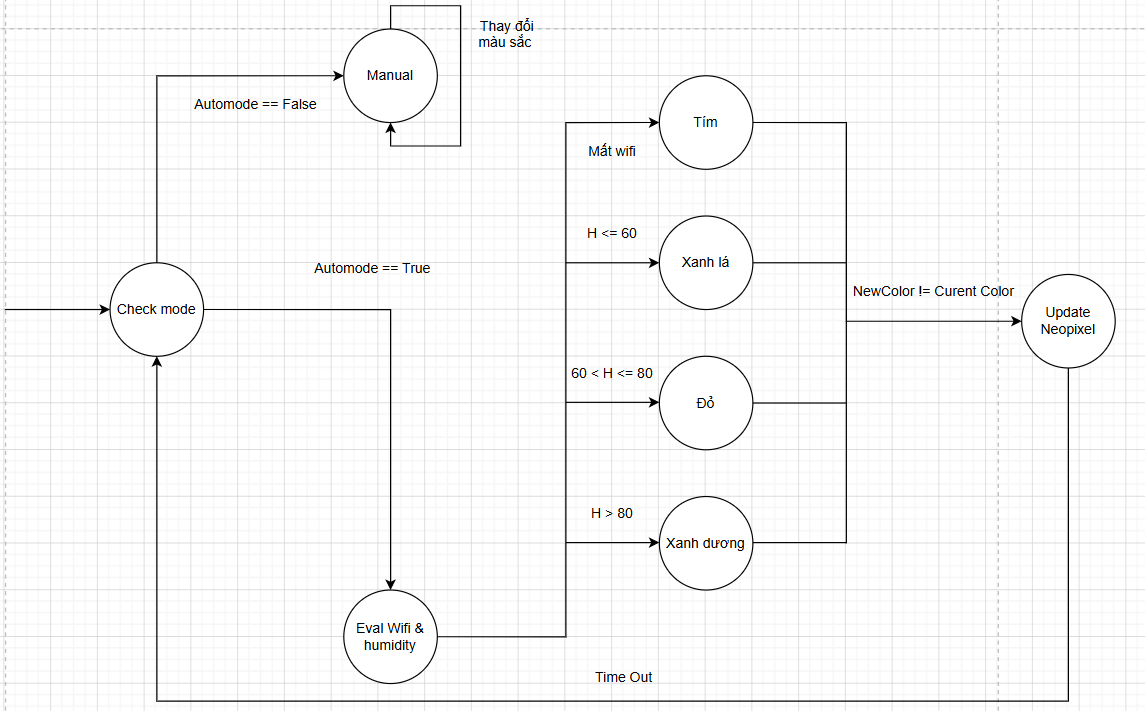
\includegraphics[width=1\linewidth]{picture/task_2_fsm.png}
 \caption{Task 2 FSM}
\end{figure}